\documentclass[11pt,a4paper]{article}
\usepackage{amsmath,amssymb,amsthm}
\usepackage{mathtools}
\usepackage{bm}
\usepackage{booktabs}
\usepackage{array}
\usepackage{enumitem}
\usepackage{geometry}
\usepackage{graphicx}
\usepackage{xcolor}
\usepackage{tcolorbox}
\usepackage{listings}
\usepackage{tikz}
\usetikzlibrary{
  arrows.meta,
  positioning,
  calc,
  shapes.geometric,
  fit,
  backgrounds
}
\usepackage[pdfencoding=auto,psdextra]{hyperref}

\geometry{margin=2.35cm}
\setlength{\emergencystretch}{3em}

\newcommand{\E}{\mathbb{E}}
\newcommand{\R}{\mathbb{R}}
\newcommand{\N}{\mathcal{N}}
\newcommand{\KL}{\mathrm{KL}}
\newcommand{\TV}{\mathrm{TV}}
\newcommand{\W}{\mathcal{W}}
\newcommand{\norm}[1]{\left\lVert #1 \right\rVert}
\newcommand{\inner}[2]{\left\langle #1,\,#2 \right\rangle}
\newcommand{\dd}{\mathrm{d}}
\newcommand{\sg}{\operatorname{sg}}
\newcommand{\old}{\mathrm{old}}
\newcommand{\fake}{\mathrm{fake}}
\newcommand{\target}{\mathrm{target}}
\newcommand{\score}{\mathsf{s}}
\newcommand{\xhat}{\widehat{x}}
\newcommand{\qks}{q_{k,\tau,s}}
\newcommand{\pkts}{p_{\theta,\tau,s}}

\theoremstyle{plain}
\newtheorem{theorem}{Theorem}[section]
\newtheorem{proposition}[theorem]{Proposition}
\newtheorem{lemma}[theorem]{Lemma}
\newtheorem{corollary}[theorem]{Corollary}

\theoremstyle{definition}
\newtheorem{definition}[theorem]{Definition}
\newtheorem{remark}[theorem]{Remark}

\definecolor{codeblue}{RGB}{32,80,150}
\definecolor{codegreen}{RGB}{30,125,70}
\definecolor{codegray}{RGB}{100,100,100}
\definecolor{codepurple}{RGB}{125,45,145}
\definecolor{oldblue}{RGB}{48,105,180}
\definecolor{teacherred}{RGB}{190,65,55}
\definecolor{studentgreen}{RGB}{45,135,90}
\definecolor{targetpurple}{RGB}{130,70,160}
\definecolor{fakeorange}{RGB}{205,120,35}

\lstdefinestyle{python}{
  language=Python,
  basicstyle=\ttfamily\small,
  keywordstyle=\color{codeblue}\bfseries,
  commentstyle=\color{codegreen},
  stringstyle=\color{codepurple},
  numbers=left,
  numberstyle=\tiny\color{codegray},
  numbersep=7pt,
  breaklines=true,
  columns=fullflexible,
  keepspaces=true,
  showstringspaces=false,
  frame=single,
  framesep=5pt,
  xleftmargin=8pt,
  framexleftmargin=6pt
}
\lstdefinestyle{badpython}{
  style=python,
  backgroundcolor=\color{red!3},
  rulecolor=\color{red!45!black}
}
\lstdefinestyle{goodpython}{
  style=python,
  backgroundcolor=\color{green!3},
  rulecolor=\color{green!45!black}
}

\tikzset{
  flowbox/.style={
    draw,
    rounded corners=2pt,
    align=center,
    minimum height=10mm,
    minimum width=27mm,
    inner sep=5pt,
    font=\small
  },
  oldbox/.style={flowbox,draw=oldblue,fill=oldblue!7},
  teacherbox/.style={flowbox,draw=teacherred,fill=teacherred!7},
  studentbox/.style={flowbox,draw=studentgreen,fill=studentgreen!7},
  targetbox/.style={flowbox,draw=targetpurple,fill=targetpurple!7},
  fakebox/.style={flowbox,draw=fakeorange,fill=fakeorange!8},
  neutralbox/.style={flowbox,draw=black!55,fill=black!3},
  decision/.style={
    diamond,
    draw=black!65,
    fill=yellow!10,
    aspect=2.1,
    align=center,
    inner sep=2pt,
    font=\small
  },
  flowarrow/.style={-{Latex[length=2.5mm]},thick,draw=black!70},
  gradarrow/.style={-{Latex[length=2.5mm]},very thick,draw=studentgreen},
  detacharrow/.style={-{Latex[length=2.5mm]},thick,dashed,draw=black!55},
  panel/.style={draw=black!25,rounded corners=3pt,fill=black!1,inner sep=7pt}
}

\title{\textbf{Mixture-of-Density DMD and TDM}\\[0.35em]
\large A strict derivation, practical surrogates, and a Flow-Factory implementation blueprint}
\author{Jayce-Ping}
\date{2026-08-03}

\begin{document}
\maketitle

\begin{abstract}
This tutorial proposes two new algorithms, \emph{Mixture-of-Density DMD} (MoD-DMD) and
\emph{Mixture-of-Density TDM} (MoD-TDM).  At outer iteration $k$, freeze the old student
$\theta_k$ and form the probability target
\[
q_{k,\tau}=(1-\alpha)\rho_{\old,\tau}+\alpha\rho_{T,\tau}.
\]
MoD-DMD minimizes a Gaussian-smoothed reverse KL at the endpoint; MoD-TDM applies the same
principle to several ODE-time marginals.  The target score is the score of the
\emph{old/teacher density mixture}, not the teacher score alone.  It can be learned without
evaluating either source density by choosing the old or teacher source once per trajectory,
adding an independent auxiliary Gaussian corruption, and training a target-mixture denoiser.

The derivation keeps two time variables separate: $\tau$ is deterministic source-ODE time,
whereas $s$ is auxiliary denoising-score-matching noise time.  We prove that smoothing preserves
mixtures, derive the smoothed responsibility, score, Tweedie denoiser, and rectified-flow
auxiliary-velocity identities with constants and signs explicit, and obtain the exact pathwise
reverse-KL gradient
\[
\E\!\left[\bar\lambda(s)\,a_s J_\theta^\top
  \bigl(\score_{\fake}-\score_q\bigr)\right].
\]
Here $\bar\lambda=\lambda/r$ includes the importance correction for the sampled auxiliary-time
density $r$.  We then derive the first-inner-step responsibility gate, both a multi-marginal
extension and a paper-style segment-conditioned TDM extension, continuous and Euler sampler
sensitivities, random-time estimators, deterministic path-law singularity, outer-loop
contraction, fitting-error bounds, and score-lag bias.

These algorithms are \textbf{proposals, not current Flow-Factory features}.  Current XDMD,
XTDM, and XOPD-DM use the frozen teacher as the real score.
They do not construct the frozen old/teacher mixture target.  The final sections map the exact
gap and give a staged implementation blueprint that preserves detach, scheduler, mixed-precision,
and distributed weight-swap invariants.
\end{abstract}

\tableofcontents
\newpage

\section{Executive summary and learning goals}
\label{sec:summary}

\subsection{The proposal in one page}

Fix a condition $C=c$ and suppress $c$ below; every distribution, score, and expectation remains
conditional on it.  At outer iteration $k$:
\begin{enumerate}[leftmargin=1.6em]
\item freeze the rollout-old source at $\theta_k$ and keep the pretrained teacher frozen;
\item define $q_{k,\tau}=(1-\alpha)\rho_{\old,\tau}+\alpha\rho_{T,\tau}$;
\item choose the source branch once per source trajectory, producing exact samples from
      $q_{k,\tau}$ at every queried $\tau$;
\item train a target-mixture score on Gaussian-corrupted source states and freeze it for the
      generator inner loop;
\item train an online fake score on detached live-student states;
\item update the student generator with the detached score difference
      $\score_{\fake}-\score_q$, backpropagated through the generated state;
\item refresh old $\leftarrow$ current only at the next outer boundary.
\end{enumerate}

MoD-DMD uses $\tau=1$.  The TDM extension has two precise readings developed below:
a TDM-inspired multi-marginal objective with an independent auxiliary channel, and a direct
segment-conditioned extension of the paper objective.  Neither is ordinary teacher DMD: the
target score is an old/teacher mixture score, not a teacher-only score.

\begin{tcolorbox}[
  colback=yellow!5,
  colframe=yellow!45!black,
  title=Status boundary]
The mathematics below specifies a future algorithm.  Current XDMD/XTDM supply the teacher as
\texttt{real}; current XOPD \texttt{marginal\_cfm} implements A4 marginal-mixture
source-velocity regression.  No current path combines the \emph{proposed} frozen mixture target
$q_{k,\tau,s}$---including an old freeze boundary and target-score phase---with DMD/TDM's online
fake-score reverse-KL update.
\end{tcolorbox}

\subsection{Learning goals}

After reading this note, the reader should be able to:
\begin{enumerate}[leftmargin=1.6em]
\item distinguish kernels, ODE fields and flows, one-time marginals, and path laws;
\item keep ODE time $\tau$ separate from auxiliary DSM time $s$;
\item derive the mixture score and rectified-flow auxiliary target without sign mistakes;
\item identify three valid target-score routes and reject source ODE velocity as a generic score;
\item derive the exact MoD-DMD and MoD-TDM pathwise gradients and their denoiser forms;
\item explain why the first inner force is responsibility gated rather than $\alpha$ times
      ordinary teacher DMD;
\item distinguish exact sampler BPTT from the current truncated one-step semi-gradient;
\item explain why deterministic path-space KL is generically singular while smoothed marginal KL
      is practical;
\item state exactly what current \texttt{XOPDTrainer}, \texttt{XDMDTrainer},
      \texttt{XTDMTrainer}, and \texttt{XOPDDMTrainer} do and what a future implementation
      must add.
\end{enumerate}

\subsection{Four probability layers and two clocks}

Figure~\ref{fig:layers-times} separates objects that are often conflated.

\begin{figure}[htbp]
\centering
\resizebox{\textwidth}{!}{
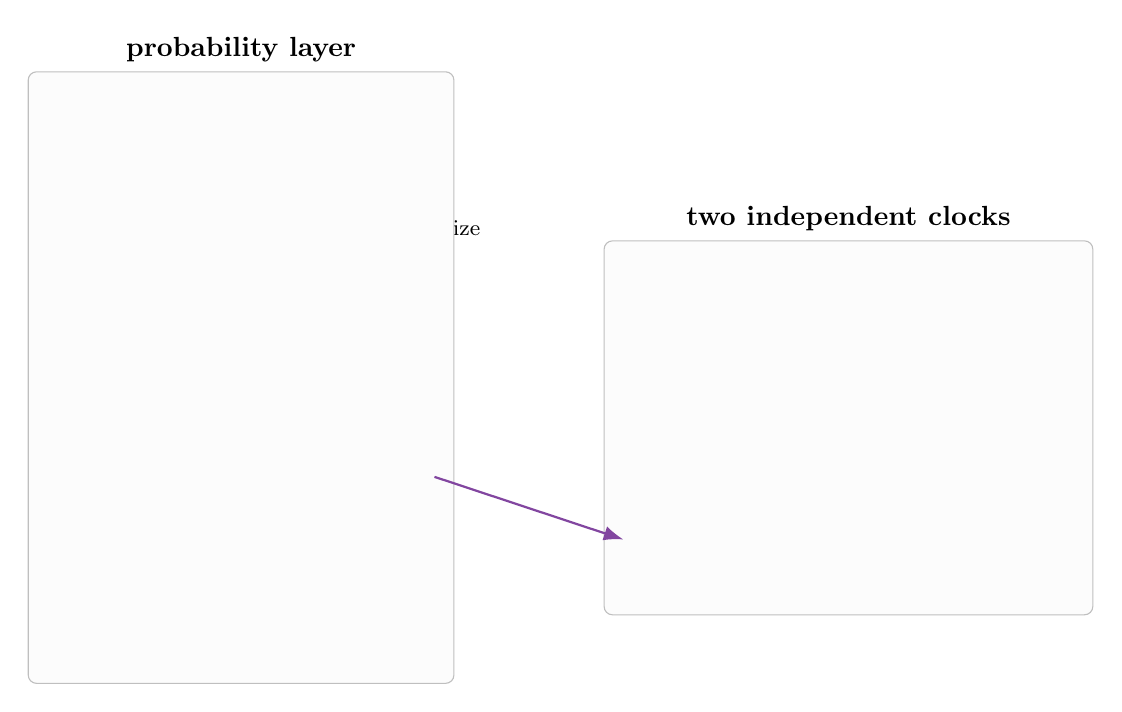
\begin{tikzpicture}[node distance=8mm and 13mm]
  \node[neutralbox,minimum width=49mm] (kernel) {
    \textbf{one-step kernel}\\$K(\dd x'\mid x)$\\stochastic transition
  };
  \node[neutralbox,minimum width=49mm,below=of kernel] (field) {
    \textbf{ODE field and flow}\\$\dot X_\tau=v_\theta(\tau,X_\tau)$\\$\Phi^\theta_{\tau\leftarrow0}$
  };
  \node[neutralbox,minimum width=49mm,below=of field] (marginal) {
    \textbf{one-time marginal}\\$\rho_{\theta,\tau}=(\Phi^\theta_{\tau\leftarrow0})_\#\rho_0$
  };
  \node[neutralbox,minimum width=49mm,below=of marginal] (path) {
    \textbf{deterministic path law}\\$\mathsf P_\theta=\mathrm{Law}\{X_\tau:0\le\tau\le1\}$
  };
  \draw[flowarrow] (field) -- node[right,font=\footnotesize] {discretize / randomize} (kernel);
  \draw[flowarrow] (field) -- node[right,font=\footnotesize] {push forward} (marginal);
  \draw[flowarrow] (field) -- node[right,font=\footnotesize,xshift=8mm] {whole graph} (path);

  \node[panel,fit=(kernel)(path),label={[font=\bfseries]above:probability layer}] {};

  \node[oldbox,right=24mm of field,minimum width=57mm] (tau) {
    \textbf{ODE trajectory time $\tau$}\\noise $\tau=0\longrightarrow$ data $\tau=1$\\
    selects $\rho_{\old,\tau},\rho_{T,\tau},p_{\theta,\tau}$
  };
  \node[targetbox,below=14mm of tau,minimum width=57mm] (s) {
    \textbf{auxiliary DSM time $s$}\\
    $Y=a_sX_\tau+b_s\varepsilon$\\
    smooths a fixed-$\tau$ marginal
  };
  \draw[flowarrow,draw=oldblue] (tau) -- node[right,font=\footnotesize] {then corrupt} (s);
  \node[panel,fit=(tau)(s),label={[font=\bfseries]above:two independent clocks}] {};
  \draw[flowarrow,draw=targetpurple] (marginal.east) -- (s.west);
\end{tikzpicture}
}
\caption{The algorithm matches Gaussian-smoothed one-time marginals.  The auxiliary corruption
clock $s$ is not the source ODE clock $\tau$, and a collection of matched marginals is not a
deterministic path-law KL.}
\label{fig:layers-times}
\end{figure}

\section{Frozen A4 outer target}
\label{sec:a4}

\subsection{Old, current, and teacher are three roles}

Let $\theta_k$ be the student checkpoint at the start of outer iteration $k$.  The rollout-old
source is frozen:
\[
\rho_{\old,\tau}:=\rho_{\theta_k,\tau}.
\]
The symbol $\theta$ denotes the trainable current student during the inner loop; after its first
optimizer step it is no longer equal to $\theta_k$.  The teacher $T$ is frozen independently.
Choose a fixed outer weight $\alpha\in[0,1]$ and define
\begin{equation}
q_{k,\tau}
:=(1-\alpha)\rho_{\old,\tau}+\alpha\rho_{T,\tau}.
\label{eq:outer-target}
\end{equation}
The complete family $\{q_{k,\tau}\}_{\tau\in[0,1]}$ is frozen during all inner updates.

\subsection{Branch once per source trajectory}

Draw $B\sim\operatorname{Bernoulli}(\alpha)$ once and initial noise $Z\sim\rho_0$.  Then
\begin{equation}
X_\tau=
\begin{cases}
\Phi^{\old}_{\tau\leftarrow0}(Z), & B=0,\\
\Phi^{T}_{\tau\leftarrow0}(Z), & B=1.
\end{cases}
\label{eq:branch-source}
\end{equation}
For every fixed $\tau$, $X_\tau\sim q_{k,\tau}$.  Keeping $B$ fixed matters: redrawing it at each
Euler step creates a switching control and approaches an arithmetic field average, not the
mixture of source-trajectory marginals.  The source path is used to sample the frozen target;
the learned student remains one deterministic generator and need not reproduce the random
source branch as a path law.

\begin{tcolorbox}[colback=blue!4,colframe=oldblue,title=Mathematical old versus the shipped A4 phase boundary]
The equations require old to remain fixed while the target score and generator inner loop are
fit.  Current \texttt{marginal\_cfm} does not materialize a separately named $\theta_k$ copy:
its $B=0$ branch calls the current student during the rollout phase, before optimization, and
then reuses cached source states and velocities.  A future target-score phase may preserve that
strict rollout-then-optimize boundary, or create an explicit snapshot if target fitting overlaps
student updates.  Reusing A4 routing alone is therefore insufficient; the freeze boundary must
also be explicit.
\end{tcolorbox}

\section{Two times: source ODE tau and auxiliary noise s}
\label{sec:two-times}

\subsection{General Gaussian corruption}

After obtaining a source or student state $X_\tau$, draw
$\varepsilon\sim\N(0,I)$ independently and set
\begin{equation}
Y=a_sX_\tau+b_s\varepsilon,
\qquad b_s>0.
\label{eq:general-corruption}
\end{equation}
The scalar $s$ indexes an auxiliary Gaussian channel.  It need not coincide with any scheduler
time used to produce $X_\tau$.  We write $\rho_{j,\tau,s}$ for the density of $Y$ when
$X_\tau\sim\rho_{j,\tau}$.

\subsection{Rectified-flow special case}

The RF corruption used in current Flow-Factory DMD helpers is
\begin{equation}
a_s=1-s,\qquad b_s=s,\qquad
Y=(1-s)X_\tau+s\varepsilon,\qquad s\in(0,1].
\label{eq:rf-corruption}
\end{equation}
Current scheduler code may represent $s$ as a decreasing noise fraction
$\sigma=t/1000$.  This is a numerical orientation convention.  It does not identify $s$ with
the source time $\tau$.

\begin{tcolorbox}[colback=red!4,colframe=red!45!black,title=Two-time warning]
The auxiliary DSM velocity
$\E[\varepsilon-X_\tau\mid Y]$ describes the conditional target of the artificial line
$Y_s=(1-s)X_\tau+s\varepsilon$.  It is \emph{not} the source ODE velocity
$v_j(\tau,X_\tau)$ that generated the clean state.
\end{tcolorbox}

\section{Smoothing, responsibilities, scores, and denoisers}
\label{sec:identities}

\subsection{Gaussian smoothing preserves mixtures}

Let
\[
\varphi_{b_s}(u)
=(2\pi b_s^2)^{-d/2}\exp\!\left(-\frac{\norm{u}^2}{2b_s^2}\right).
\]
For source $j\in\{\old,T\}$,
\begin{equation}
\rho_{j,\tau,s}(y)
=\int_{\R^d}\varphi_{b_s}(y-a_sx)\rho_{j,\tau}(x)\dd x.
\label{eq:smoothed-source}
\end{equation}

\begin{proposition}[Linearity of smoothing]
\label{prop:smoothing-mixture}
The smoothed A4 target is
\begin{equation}
q_{k,\tau,s}(y)
=(1-\alpha)\rho_{\old,\tau,s}(y)
+\alpha\rho_{T,\tau,s}(y).
\label{eq:smoothed-mixture}
\end{equation}
\end{proposition}

\begin{proof}
Insert \eqref{eq:outer-target} into the convolution integral and use linearity:
\[
\int\varphi_{b_s}(y-a_sx)
\bigl[(1-\alpha)\rho_{\old,\tau}(x)+\alpha\rho_{T,\tau}(x)\bigr]\dd x
=(1-\alpha)\rho_{\old,\tau,s}(y)+\alpha\rho_{T,\tau,s}(y).
\]
\end{proof}

\subsection{Smoothed responsibility and mixture-score identity}

Where $q_{k,\tau,s}(y)>0$, define exactly
\begin{equation}
\boxed{
\gamma_{k,\tau,s}(y)
:=\frac{\alpha\rho_{T,\tau,s}(y)}{q_{k,\tau,s}(y)}
}.
\label{eq:smoothed-gamma}
\end{equation}
This is the posterior probability $\Pr(B=1\mid Y=y,\tau,s)$.  It is neither A4's unsmoothed
responsibility $\alpha\rho_{T,\tau}/q_{k,\tau}$ nor an SDE transition gate.

\begin{proposition}[Mixture score]
\label{prop:mixture-score}
Writing $\score_j=\nabla_y\log\rho_{j,\tau,s}$ and
$\score_q=\nabla_y\log q_{k,\tau,s}$,
\begin{equation}
\boxed{
\score_q(y)
=\bigl(1-\gamma_{k,\tau,s}(y)\bigr)\score_{\old}(y)
+\gamma_{k,\tau,s}(y)\score_T(y)
}.
\label{eq:mixture-score}
\end{equation}
\end{proposition}

\begin{proof}
Differentiate \eqref{eq:smoothed-mixture}, use
$\nabla\rho_j=\rho_j\score_j$, and divide by $q_{k,\tau,s}$.
\end{proof}

\subsection{Tweedie's identity with all constants}

\begin{proposition}[General Gaussian score and denoiser {\cite{tweedie}}]
\label{prop:tweedie}
For $Y=a_sX+b_s\varepsilon$ with $b_s>0$,
\begin{equation}
\boxed{
\nabla_y\log p_s(y)
=\frac{a_s\E[X\mid Y=y]-y}{b_s^2}
}.
\label{eq:general-score}
\end{equation}
If $a_s\ne0$, the posterior-mean clean estimate is
\begin{equation}
\boxed{
\xhat_p(y,s):=\E[X\mid Y=y]
=\frac{y+b_s^2\score_p(y,s)}{a_s}
}.
\label{eq:general-denoiser}
\end{equation}
\end{proposition}

\begin{proof}
Differentiate under the integral:
\begin{align*}
\nabla_y p_s(y)
&=\int-\frac{y-a_sx}{b_s^2}
  \varphi_{b_s}(y-a_sx)p(x)\dd x\\
&=\frac{a_s\E[X\mid Y=y]-y}{b_s^2}\,p_s(y).
\end{align*}
Division by $p_s(y)$ proves \eqref{eq:general-score}; rearranging proves
\eqref{eq:general-denoiser}.
\end{proof}

\subsection{RF auxiliary velocity: sign check}

Under \eqref{eq:rf-corruption}, define
\begin{equation}
d_p(y,s):=\E[\varepsilon-X\mid Y=y].
\label{eq:rf-d}
\end{equation}
Because $Y=X+s(\varepsilon-X)$,
\begin{equation}
\boxed{\xhat_p(y,s)=\E[X\mid Y=y]=y-s\,d_p(y,s)}.
\label{eq:rf-xhat}
\end{equation}
Substituting $a_s=1-s$, $b_s=s$ and \eqref{eq:rf-xhat} into
\eqref{eq:general-score} gives
\begin{align}
\score_p(y,s)
&=\frac{(1-s)(y-sd_p)-y}{s^2}\nonumber\\
&=\boxed{-\frac{y+(1-s)d_p(y,s)}{s}}.
\label{eq:rf-score}
\end{align}
Both the minus sign and the factor $(1-s)$ are essential.  A denoising regression
\[
\E\norm{d_\eta(Y,\tau,s)-(\varepsilon-X_\tau)}^2
\]
has population minimizer $d_p$; it does not estimate $v(\tau,\cdot)$.

\section{Three routes to the frozen target-mixture score}
\label{sec:routes}

\subsection{Route A: branch-sampled target score/FM loss (preferred)}

Sample $B$ once per source trajectory, query $X_\tau$ on that trajectory, corrupt it with fresh
$(s,\varepsilon)$, and regress a target network onto the auxiliary label.  Marginalizing $B$
produces $X_\tau\sim q_{k,\tau}$; ordinary conditional regression therefore learns the
posterior-averaged $d_q$ or equivalent score.  No density or classifier is evaluated.

\begin{figure}[htbp]
\centering
\resizebox{\textwidth}{!}{
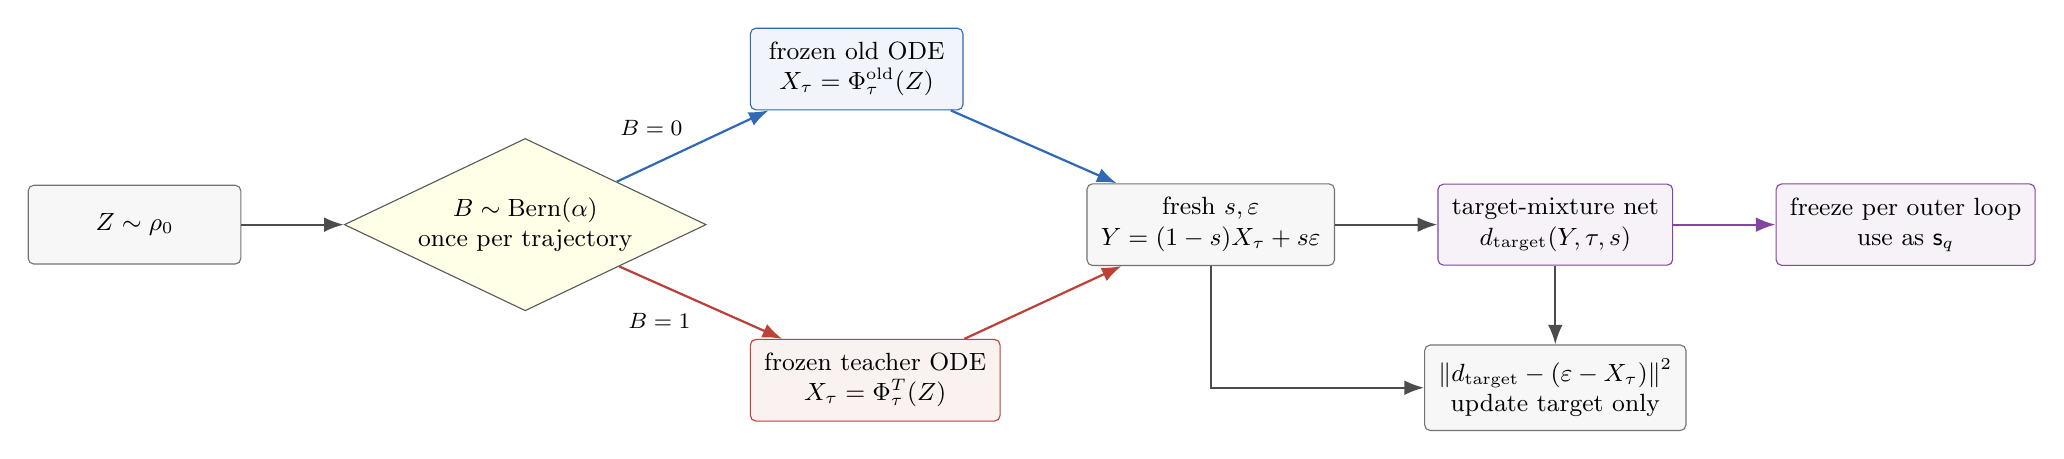
\begin{tikzpicture}[node distance=10mm and 13mm]
  \node[neutralbox] (z) {$Z\sim\rho_0$};
  \node[decision,right=of z] (b) {$B\sim\mathrm{Bern}(\alpha)$\\once per trajectory};
  \node[oldbox,above right=9mm and 17mm of b] (oldflow) {
    frozen old ODE\\$X_\tau=\Phi^\old_\tau(Z)$
  };
  \node[teacherbox,below right=9mm and 17mm of b] (tflow) {
    frozen teacher ODE\\$X_\tau=\Phi^T_\tau(Z)$
  };
  \node[neutralbox,right=28mm of $(oldflow)!0.5!(tflow)$] (noise) {
    fresh $s,\varepsilon$\\$Y=(1-s)X_\tau+s\varepsilon$
  };
  \node[targetbox,right=of noise] (net) {
    target-mixture net\\$d_{\target}(Y,\tau,s)$
  };
  \node[neutralbox,below=of net] (loss) {
    $\norm{d_{\target}-(\varepsilon-X_\tau)}^2$\\
    update target only
  };
  \node[targetbox,right=of net] (freeze) {
    freeze per outer loop\\use as $\score_q$
  };
  \draw[flowarrow] (z) -- (b);
  \draw[flowarrow,draw=oldblue] (b) -- node[above left,font=\footnotesize] {$B=0$} (oldflow);
  \draw[flowarrow,draw=teacherred] (b) -- node[below left,font=\footnotesize] {$B=1$} (tflow);
  \draw[flowarrow,draw=oldblue] (oldflow) -- (noise);
  \draw[flowarrow,draw=teacherred] (tflow) -- (noise);
  \draw[flowarrow] (noise) -- (net);
  \draw[flowarrow] (noise) |- (loss);
  \draw[flowarrow] (net) -- (loss);
  \draw[flowarrow,draw=targetpurple] (net) -- (freeze);
\end{tikzpicture}
}
\caption{Preferred RF target-score training.  The source branch generates the correct target
marginal; the auxiliary Gaussian channel supplies a standard DSM/FM label.  The resulting
target-mixture score is frozen during generator inner updates.}
\label{fig:target-training}
\end{figure}

\subsection{Route B: responsibility classifier plus source scores}

Train a calibrated classifier $r_\xi(y,\tau,s)\approx\Pr(B=1\mid y,\tau,s)$ and source score
models $\widehat\score_{\old}$, $\widehat\score_T$.  Then use
\[
\widehat\score_q=(1-r_\xi)\widehat\score_{\old}+r_\xi\widehat\score_T.
\]
This route is analytically transparent and exposes $\gamma_{k,\tau,s}$ for diagnostics, but it
requires three accurate learned objects.  When source scores differ greatly,
small classifier error is amplified.

\subsection{Route C: mixture-versus-current density ratio}

Train a discriminator between $Y_q\sim q_{k,\tau,s}$ and
$Y_p\sim p_{\theta,\tau,s}$.  With equal class priors and optimal logit
$\ell^\star=\log q_{k,\tau,s}-\log p_{\theta,\tau,s}$,
\begin{equation}
\nabla_y\ell^\star(y)=\score_q(y)-\score_{\fake}(y).
\label{eq:ratio-force}
\end{equation}
This directly estimates the force needed by reverse KL, but it must track the moving current
student and can be ill-conditioned when the two densities have little overlap.

\subsection{Why source ODE velocity is not a marginal score}

The continuity equation
\[
\partial_\tau\rho_\tau+\nabla\!\cdot(\rho_\tau v_\tau)=0
\]
does not determine $\nabla\log\rho_\tau$ from the local value $v_\tau(x)$.  The score depends on
the global transported density and the flow Jacobian.  A probability-flow ODE can be related to a
score only after specifying a particular forward diffusion and drift/diffusion coefficients.
Therefore neither $v_{\old}(\tau,x)$ nor $v_T(\tau,x)$ may be substituted for the score of the
intermediate marginal $\rho_{j,\tau,s}$ without a separate proof.

\begin{lstlisting}[style=badpython,caption={Wrong: source ODE velocity is not a generic DSM score.}]
# X_tau was produced by the source ODE at trajectory time tau.
score_q = (1 - alpha) * old.velocity(tau, X_tau) \
        + alpha * teacher.velocity(tau, X_tau)
loss = dmd_surrogate(score_fake - score_q)
\end{lstlisting}

\begin{lstlisting}[style=goodpython,caption={Correct conceptual target-score sampling.}]
# branch is sampled once and held fixed for the complete source trajectory.
X_tau = frozen_source_trajectory(branch).state_at(tau)
epsilon = torch.randn_like(X_tau)
Y = a(s) * X_tau + b(s) * epsilon
aux_target = epsilon - X_tau                  # RF auxiliary velocity label
loss_target = mse(target_net(Y, tau, s), aux_target)
\end{lstlisting}

\section{Endpoint MoD-DMD}
\label{sec:mod-dmd}

\subsection{Smoothed reverse-KL objective}

Let $X=G_\theta(Z)$ be the current endpoint sample and let $p_{\theta,1,s}$ be the density of
$Y=a_sX+b_s\varepsilon$.  For a nonnegative integrable weight $\lambda(s)$, define
\begin{equation}
\mathcal L_{\mathrm{MoD\text{-}DMD}}(\theta;q_k)
=\int_{\mathcal S}\lambda(s)
\KL\!\left(p_{\theta,1,s}\Vert q_{k,1,s}\right)\dd s.
\label{eq:mod-dmd-objective}
\end{equation}
In Monte Carlo, draw $S\sim r$ from a density that is positive wherever $\lambda$ is nonzero and
write $\bar\lambda(S):=\lambda(S)/r(S)$.  The target $q_k$ is held fixed while differentiating.
This is the mixture-target counterpart of score-based implicit-distribution matching used by
Diff-Instruct and DMD/DMD2~\cite{diffinstruct,dmd,dmd2}.

The displayed $G_\theta$ is sampler-agnostic.  Current \texttt{XDMDTrainer} instantiates it as a
DMD2 consistency-style backward simulation: a no-grad predict-$x_0$/fresh-re-noise prefix and
one differentiable clean prediction, rather than a differentiable ODE endpoint.

\subsection{Exact pathwise reverse-KL gradient}

Write $J_\theta(Z)=\partial G_\theta(Z)/\partial\theta$ and
\[
\score_{\fake}(y,s)=\nabla_y\log p_{\theta,1,s}(y),
\qquad
\score_q(y,s)=\nabla_y\log q_{k,1,s}(y).
\]

\begin{theorem}[Pathwise MoD-DMD gradient]
\label{thm:dmd-gradient}
Under the usual differentiability, integrability, and vanishing-boundary conditions,
\begin{equation}
\boxed{
\nabla_\theta\mathcal L_{\mathrm{MoD\text{-}DMD}}
=\E_{Z,\varepsilon,s}\!\left[
\bar\lambda(s)\,a_sJ_\theta(Z)^\top
\bigl(\score_{\fake}(Y,s)-\score_q(Y,s)\bigr)
\right].
}
\label{eq:pathwise-gradient}
\end{equation}
Thus gradient descent moves samples in the direction
$\score_q-\score_{\fake}$.
\end{theorem}

\begin{proof}
For one $s$, differentiate the reparameterized expectation of
$\log p_{\theta,1,s}(Y)-\log q_{k,1,s}(Y)$.  The pathwise derivative through $Y$ contributes
$(\score_{\fake}-\score_q)^\top\partial_\theta Y$.  The expected explicit parameter derivative
of $\log p_{\theta,1,s}$ vanishes by score normalization.  Since
$\partial_\theta Y=a_sJ_\theta$, sampling $s$ with the factor
$\bar\lambda(s)=\lambda(s)/r(s)$ gives the integral in
\eqref{eq:pathwise-gradient}.
\end{proof}

\subsection{Denoiser form and timestep weights}

From \eqref{eq:general-denoiser},
\begin{equation}
\score_{\fake}-\score_q
=\frac{a_s}{b_s^2}
\bigl(\xhat_{\fake}-\xhat_q\bigr).
\label{eq:score-to-denoiser}
\end{equation}
Therefore
\begin{equation}
\boxed{
\nabla_\theta\mathcal L_{\mathrm{MoD\text{-}DMD}}
=\E\!\left[
\bar\lambda(s)\frac{a_s^2}{b_s^2}
J_\theta^\top(\xhat_{\fake}-\xhat_q)
\right].
}
\label{eq:denoiser-gradient}
\end{equation}
Using the bare clean-estimate residual
$\xhat_{\fake}-\xhat_q$ is legitimate only as a deliberately reweighted surrogate: it replaces
the exact effective weight $\lambda(s)a_s^2/b_s^2$ by another timestep weighting.

For RF, \eqref{eq:rf-xhat} gives
\[
\xhat_{\fake}-\xhat_q=-s(d_{\fake}-d_q).
\]
Again, a bare auxiliary-velocity residual changes the $s$ weighting unless the compensating
factor is included.

\subsection{Online fake loss and detach boundaries}

The fake network estimates the score of the \emph{live} student distribution.  Generate a current
endpoint $X_\theta$, detach it, add fresh auxiliary noise, and optimize
\begin{equation}
\mathcal L_{\fake}(\phi)
=\E\norm{d_\phi(Y,s)-(\varepsilon-\sg X_\theta)}^2.
\label{eq:fake-loss}
\end{equation}
During generator backward, both target and fake predictions are detached.  Only
$X_\theta=G_\theta(Z)$ retains a generator graph.

\begin{lstlisting}[style=goodpython,caption={Conceptual endpoint generator update with exact detach roles.}]
X = student_generator(noise, condition)          # keeps generator graph
s, epsilon = sample_auxiliary_corruption(X.detach())
Y_value = a(s) * X.detach() + b(s) * epsilon     # score-query value

with torch.no_grad():
    score_q = frozen_target_mixture.score(Y_value, tau=1.0, s=s)
    score_fake = online_fake.score(Y_value, tau=1.0, s=s)
    force = importance_weight(s) * a(s) * (score_fake - score_q)

# d(loss)/dX equals detached force; only X backpropagates.
target = (X.float() - force.float()).detach()
loss_gen = 0.5 * event_reduce((X.float() - target).square())
loss_gen.backward()
\end{lstlisting}

\subsection{Event sum, event mean, self-normalization, and Pseudo-Huber}

For event dimension $D$, the exact Euclidean inner product corresponds to an event sum.
An event mean multiplies the complete gradient by $1/D$ at fixed shape, preserving stationary
points but changing resolution-dependent optimization scale.  It should be documented as a
normalization, not as a different KL.

DMD2-style self-normalization divides the detached force by a sample-dependent scale such as
$\operatorname{mean}|p_{\target}|$.  This generally changes relative weighting across examples
and timesteps; it is a stability heuristic, not the exact gradient of
\eqref{eq:mod-dmd-objective}.  Pseudo-Huber similarly rescales large residuals.  It can stabilize
heavy-tailed forces, but its gradient is not the unmodified reverse-KL force unless the induced
scalar multiplier is explicitly included in the intended objective.

\begin{tcolorbox}[
  colback=green!5,
  colframe=green!50!black,
  title=Algorithm 1: one outer iteration of proposed MoD-DMD]
\begin{enumerate}[leftmargin=1.6em]
\item Snapshot $\theta_k$ as the frozen rollout-old source.
\item Sample complete old/teacher source trajectories with one Bernoulli branch per trajectory.
\item Train the target-mixture DSM/FM network on $(X_1,s,\varepsilon)$; then freeze it.
\item Repeatedly train the online fake score on detached live-student endpoints.
\item For each generator update, retain the student sampler graph, query both scores under
      no-grad, construct the detached force
      $\bar\lambda(s)a_s(\score_{\fake}-\score_q)$, and backpropagate only through the endpoint.
\item At the next outer boundary, evaluate fitting diagnostics and refresh old
      $\leftarrow\theta$.
\end{enumerate}
\end{tcolorbox}

\section{The first inner step is responsibility gated}
\label{sec:first-step}

\begin{theorem}[First-inner-step force]
\label{thm:first-step}
Suppose the inner loop begins with
$p_{\theta,\tau,s}=\rho_{\old,\tau,s}$ under the same Gaussian channel and the score estimates
are exact.  Then
\begin{equation}
\score_{\fake}-\score_q
=\gamma_{k,\tau,s}\bigl(\score_{\old}-\score_T\bigr),
\label{eq:first-gradient}
\end{equation}
so the negative-gradient sample force is
\begin{equation}
\boxed{
\score_q-\score_{\fake}
=\gamma_{k,\tau,s}\bigl(\score_T-\score_{\old}\bigr).
}
\label{eq:first-force}
\end{equation}
\end{theorem}

\begin{proof}
At initialization $\score_{\fake}=\score_{\old}$.  Substitute
\eqref{eq:mixture-score} and simplify.
\end{proof}

The gate is the \emph{smoothed posterior responsibility}
$\gamma_{k,\tau,s}(y)$, not the prior $\alpha$.  Therefore the first step is not
``$\alpha$ times teacher DMD.''  Where teacher density is negligible, reverse KL gives little
teacher-directed force even if $\alpha$ is moderate.  Increasing auxiliary smoothing increases
overlap and softens the responsibility boundary, but excessive smoothing removes fine target
structure.

Reverse KL is mode seeking: a finite-capacity student may concentrate on a subset of mixture
modes rather than representing the full convex mixture.  One optimizer step only takes a local
parameter-space move under $J_\theta$; it does not set $p_\theta=q_k$.  Exact realization of
$q_k$ requires sufficient capacity, score accuracy, sampler sensitivity, and inner optimization.

\section{MoD-TDM: multi-time and segment-conditioned matching}
\label{sec:mod-tdm}

\subsection{TDM-inspired multi-marginal objective}

Choose trajectory times $0<\tau_1<\cdots<\tau_m\le1$ and weights $w_i\ge0$.  Define
\begin{equation}
\mathcal L_{\mathrm{MoD\text{-}TDM}}(\theta;q_k)
=\sum_{i=1}^m w_i
\int_{\mathcal S}\lambda_i(s)
\KL\!\left(p_{\theta,\tau_i,s}\Vert q_{k,\tau_i,s}\right)\dd s.
\label{eq:mod-tdm-objective}
\end{equation}
Endpoint MoD-DMD is the special case $m=1$, $\tau_1=1$.
The multi-time construction is motivated by trajectory distribution matching~\cite{tdm}, but
its real target here is the frozen old/teacher mixture rather than the teacher alone.

If $I\sim\pi$ with $\pi_i>0$, then
\begin{equation}
\E_I\!\left[
\frac{w_I}{\pi_I}\,
\nabla_\theta\int\lambda_I(s)
\KL(p_{\theta,\tau_I,s}\Vert q_{k,\tau_I,s})\dd s
\right]
=\nabla_\theta\mathcal L_{\mathrm{MoD\text{-}TDM}}.
\label{eq:random-time-unbiased}
\end{equation}
Uniform random segment selection is unbiased for a uniform sum only when the corresponding
$m$ factor is included; omitting it merely rescales the whole objective if all other weights are
equal, but nonuniform sampling requires $w_i/\pi_i$.  Likewise, sampling
$S\sim r_i$ inside the chosen term requires $\lambda_i(S)/r_i(S)$.

\begin{figure}[htbp]
\centering
\resizebox{\textwidth}{!}{
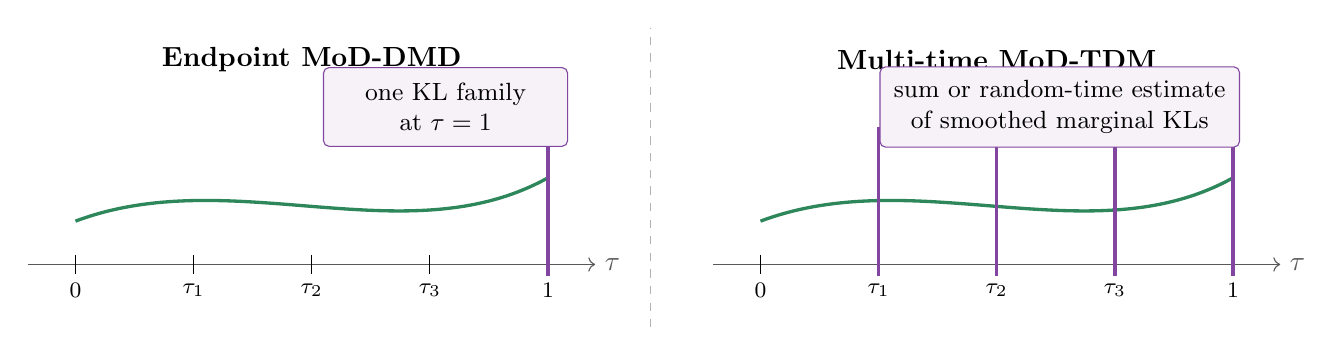
\begin{tikzpicture}[x=1cm,y=1cm]
  \node[font=\bfseries] at (0,2.6) {Endpoint MoD-DMD};
  \draw[->,black!65] (-3.6,0) -- (3.6,0) node[right] {$\tau$};
  \foreach \x/\lab in {-3/0,-1.5/{\tau_1},0/{\tau_2},1.5/{\tau_3},3/1}
    \draw (\x,0.12)--(\x,-0.12) node[below,font=\footnotesize] {$\lab$};
  \draw[very thick,studentgreen] (-3,0.55) .. controls (-1,1.3) and (1.2,0.1) .. (3,1.1);
  \draw[targetpurple,very thick] (3,-0.15) -- (3,1.75);
  \node[targetbox,minimum width=31mm] at (1.7,2.0) {one KL family\\at $\tau=1$};

  \draw[dashed,black!30] (4.3,-0.8) -- (4.3,3.0);

  \begin{scope}[xshift=8.7cm]
    \node[font=\bfseries] at (0,2.6) {Multi-time MoD-TDM};
    \draw[->,black!65] (-3.6,0) -- (3.6,0) node[right] {$\tau$};
    \foreach \x/\lab in {-3/0,-1.5/{\tau_1},0/{\tau_2},1.5/{\tau_3},3/1}
      \draw (\x,0.12)--(\x,-0.12) node[below,font=\footnotesize] {$\lab$};
    \draw[very thick,studentgreen] (-3,0.55) .. controls (-1,1.3) and (1.2,0.1) .. (3,1.1);
    \foreach \x in {-1.5,0,1.5,3}
      \draw[targetpurple,very thick] (\x,-0.15) -- (\x,1.75);
    \node[targetbox,minimum width=42mm] at (0.8,2.0) {sum or random-time estimate\\of smoothed marginal KLs};
  \end{scope}
\end{tikzpicture}
}
\caption{Endpoint DMD constrains one generated marginal.  TDM distributes score-difference
forces across trajectory times.  The vertical bars denote auxiliary-smoothed marginal KL
families, not deterministic path-space KL.}
\label{fig:endpoint-vs-tdm}
\end{figure}

\subsection{Direct extension of the paper-style segment objective}
\label{sec:segment-mod-tdm}

Equation~\eqref{eq:mod-tdm-objective} is best described as
\emph{TDM-inspired multi-marginal DMD}: it first selects a clean student/source marginal at
$\tau_i$ and then applies an independently indexed auxiliary channel $K_s$ to both sides.
Paper-style TDM instead anchors at a segment boundary and uses the native forward kernel over a
non-overlapping segment.  Let $I_i$ be the $i$th segment and let
$K_{u\mid\tau_i}$ denote that kernel for $u\in I_i$.  Define
\begin{equation}
p_{\theta,u}^{(i)}
:=(K_{u\mid\tau_i})_\#p_{\theta,\tau_i},
\qquad
q_{k,u}:=(1-\alpha)\rho_{\old,u}+\alpha\rho_{T,u}.
\label{eq:native-segment-target}
\end{equation}
The paper-faithful mixture-target replacement is
\begin{equation}
\boxed{
\mathcal L_{\mathrm{native\text{-}seg\text{-}MoD\text{-}TDM}}
:=\sum_i\int_{u\in I_i}\lambda_i(u)
\KL\!\left(p_{\theta,u}^{(i)}\Vert q_{k,u}\right)\dd u.
}
\label{eq:segment-mod-tdm}
\end{equation}
Here the target is the native-time source mixture at $u$; branch-fixed old/teacher trajectories
provide direct samples from it.  Samples alone do not provide an exact score label.  The native
$\score_q(\cdot,u)$ therefore requires either valid source native-time scores plus a responsibility
estimator, an explicit score-matching method, or another justified estimator.  Applying an
additional DSM corruption is often practical, but it changes the target to a further-smoothed
native segment law and must be written as such.

A second, valid but different construction symmetrically applies the segment kernel to the
anchor target:
\begin{align}
\widetilde q_{k,u}^{(i)}
&:=(K_{u\mid\tau_i})_\#q_{k,\tau_i}\nonumber\\
&=(1-\alpha)(K_{u\mid\tau_i})_\#\rho_{\old,\tau_i}
  +\alpha(K_{u\mid\tau_i})_\#\rho_{T,\tau_i}.
\label{eq:symmetric-segment-mixture}
\end{align}
Linearity preserves the mixture, so branch sampling also trains this score.  The native target
$q_{k,u}$ and symmetric target $\widetilde q_{k,u}^{(i)}$ coincide only when each source is
consistent with that same kernel,
\[
(K_{u\mid\tau_i})_\#\rho_{j,\tau_i}=\rho_{j,u},
\qquad j\in\{\old,T\},
\]
and should otherwise be named as different objectives.

For a reparameterized segment kernel
$Y_u=T_{u\mid\tau_i}(X_{\tau_i},\varepsilon)$, the native-target gradient is
\begin{equation}
\nabla_\theta\mathcal L_{\mathrm{native\text{-}seg}}
=\sum_i\int_{I_i}\lambda_i(u)\,
\E\!\left[
S_\theta(\tau_i)^\top D_xT_{u\mid\tau_i}^{\top}
\bigl(\score_{\fake}^{(i)}(Y_u,u)-\score_q(Y_u,u)\bigr)
\right]\dd u.
\label{eq:segment-gradient}
\end{equation}
If $I\sim\pi$ and $U\sim r_I$, its Monte Carlo multiplier is
$\lambda_I(U)/[\pi_Ir_I(U)]$.  For an affine kernel
$Y_u=a_{i,u}X_{\tau_i}+b_{i,u}\varepsilon$, the Jacobian factor reduces to
$a_{i,u}S_\theta(\tau_i)^\top$.

Thus \eqref{eq:mod-tdm-objective} and \eqref{eq:segment-mod-tdm} are related but not identical.
They coincide only after identifying $K_s$ with $K_{u\mid\tau_i}$, matching the sampling
measures, and establishing the required target identities.  Current Flow-Factory
\texttt{XTDMTrainer} follows a practical segment-banded surrogate: it treats the selected
post-Euler state as a clean anchor, re-noises it in the segment's non-overlapping scheduler band,
and queries teacher/fake denoisers.  That engineering rule is not automatically the independent
two-clock objective \eqref{eq:mod-tdm-objective}.

\subsection{Continuous ODE sensitivity}

For noise-to-data orientation,
\begin{equation}
\frac{\dd X_\theta(\tau)}{\dd\tau}
=v_\theta(\tau,X_\theta(\tau)),
\qquad X_\theta(0)=Z.
\label{eq:student-ode}
\end{equation}
Let $S_\theta(\tau)=\partial_\theta X_\theta(\tau)$.  Differentiating gives
\begin{equation}
\frac{\dd S_\theta}{\dd\tau}
=\partial_xv_\theta(\tau,X_\theta)S_\theta
+\partial_\theta v_\theta(\tau,X_\theta),
\qquad S_\theta(0)=0.
\label{eq:continuous-sensitivity}
\end{equation}
The exact marginal gradient at $\tau_i$ contains
$a_sS_\theta(\tau_i)^\top(\score_{\fake}-\score_q)$.

\subsection{Euler sensitivity and scheduler orientation}

For an increasing mathematical grid with $h_i=\tau_{i+1}-\tau_i>0$,
\begin{align}
X_{i+1}&=X_i+h_iv_\theta(\tau_i,X_i),\label{eq:euler-state}\\
S_{i+1}
&=\bigl(I+h_i\partial_xv_\theta(\tau_i,X_i)\bigr)S_i
+h_i\partial_\theta v_\theta(\tau_i,X_i).
\label{eq:euler-sensitivity}
\end{align}
FLUX-style scheduler code often uses decreasing $\sigma_i$.  Its actual update is
\begin{equation}
X_{i+1}=X_i+(\sigma_{i+1}-\sigma_i)v_\theta(\sigma_i,X_i),
\qquad \sigma_{i+1}-\sigma_i<0.
\label{eq:scheduler-step}
\end{equation}
The sensitivity must use this signed increment.  Silently replacing it by
$|\sigma_{i+1}-\sigma_i|$ reverses the generator Jacobian contribution.

\subsection{Exact BPTT versus current truncated semi-gradient}

Exact BPTT retains all terms in \eqref{eq:euler-sensitivity}.  The current XTDM v1 pattern rolls
out the prefix under \texttt{no\_grad} and keeps only one selected Euler step differentiable.  If
$X_i$ is detached, then
\begin{equation}
S_{i+1}^{\mathrm{trunc}}
=(\sigma_{i+1}-\sigma_i)
\partial_\theta v_\theta(\sigma_i,\sg X_i).
\label{eq:truncated-sensitivity}
\end{equation}
It omits the sensitivity of all earlier steps and the propagation term
$(I+\Delta\sigma_i\partial_xv_i)S_i$.  It is a memory-efficient truncated
\emph{semi-gradient}, not the exact gradient of the full multi-time objective.

\begin{figure}[htbp]
\centering
\resizebox{\textwidth}{!}{
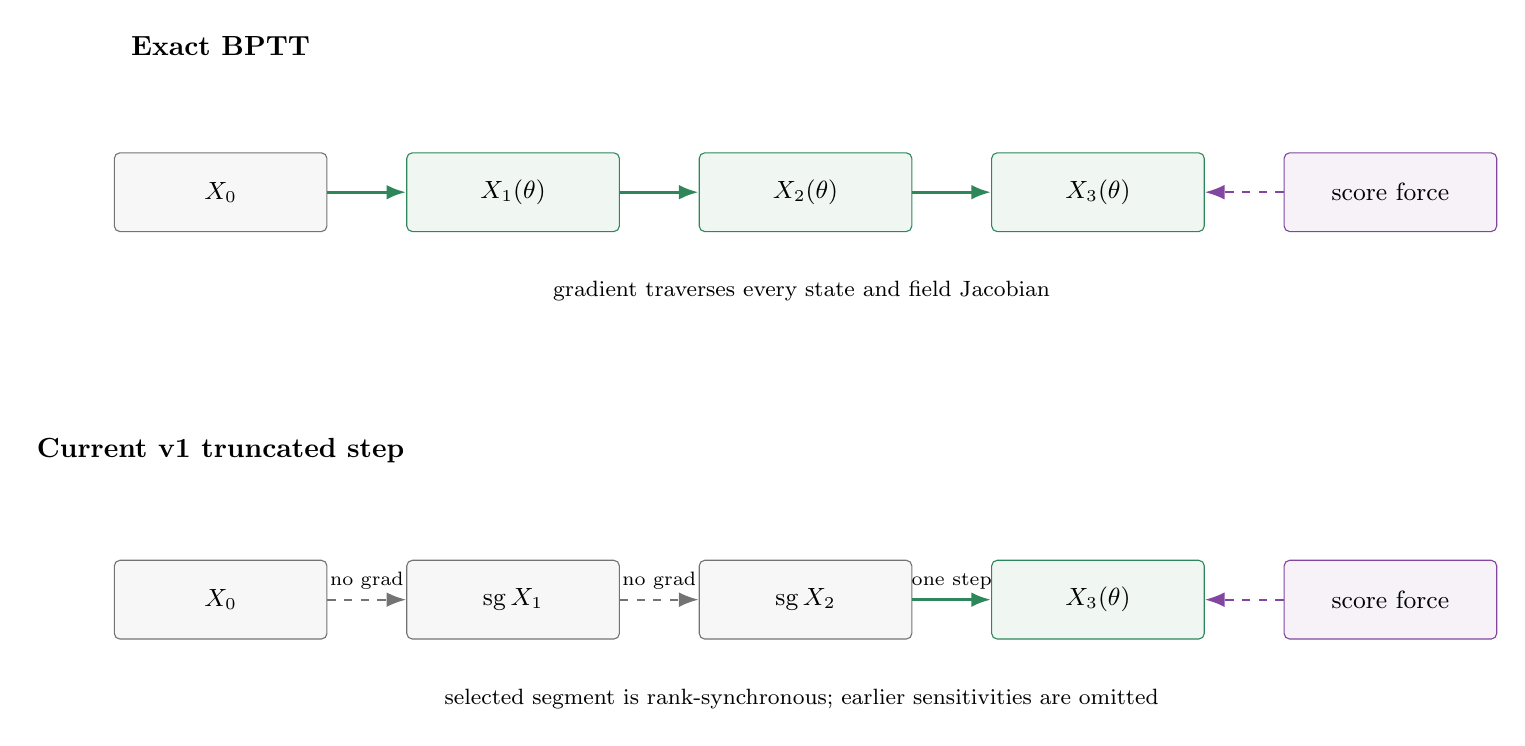
\begin{tikzpicture}[node distance=11mm and 10mm]
  \node[font=\bfseries] (et) {Exact BPTT};
  \node[neutralbox,below=of et] (e0) {$X_0$};
  \node[studentbox,right=of e0] (e1) {$X_1(\theta)$};
  \node[studentbox,right=of e1] (e2) {$X_2(\theta)$};
  \node[studentbox,right=of e2] (e3) {$X_3(\theta)$};
  \node[targetbox,right=of e3] (ef) {score force};
  \draw[gradarrow] (e0)--(e1);
  \draw[gradarrow] (e1)--(e2);
  \draw[gradarrow] (e2)--(e3);
  \draw[detacharrow,draw=targetpurple] (ef)--(e3);
  \node[font=\footnotesize,align=center,below=5mm of e2] {
    gradient traverses every state and field Jacobian
  };

  \node[font=\bfseries,below=25mm of e0] (tt) {Current v1 truncated step};
  \node[neutralbox,below=of tt] (t0) {$X_0$};
  \node[neutralbox,right=of t0] (t1) {$\sg X_1$};
  \node[neutralbox,right=of t1] (t2) {$\sg X_2$};
  \node[studentbox,right=of t2] (t3) {$X_3(\theta)$};
  \node[targetbox,right=of t3] (tf) {score force};
  \draw[detacharrow] (t0)--node[above,font=\scriptsize]{no grad}(t1);
  \draw[detacharrow] (t1)--node[above,font=\scriptsize]{no grad}(t2);
  \draw[gradarrow] (t2)--node[above,font=\scriptsize]{one step}(t3);
  \draw[detacharrow,draw=targetpurple] (tf)--(t3);
  \node[font=\footnotesize,align=center,below=5mm of t2] {
    selected segment is rank-synchronous; earlier sensitivities are omitted
  };
\end{tikzpicture}
}
\caption{Exact sampler sensitivity versus the current no-grad-prefix plus one differentiable
step approximation.  The score force is detached in both cases; the difference is the state
Jacobian retained by the generator.}
\label{fig:jacobians}
\end{figure}

\section{Why practical TDM is not deterministic path-space KL}
\label{sec:path-singularity}

On a grid $\tau_0,\ldots,\tau_m$, a deterministic ODE maps one initial state $z\in\R^d$ to
\[
F_\theta(z)
=\bigl(z,\Phi^\theta_{\tau_1}(z),\ldots,\Phi^\theta_{\tau_m}(z)\bigr)
\in\R^{d(m+1)}.
\]
The path law is supported on the $d$-dimensional graph
$\mathcal G_\theta=\{F_\theta(z):z\in\R^d\}$.

\begin{proposition}[Generic path-law singularity]
\label{prop:path-singularity}
For two deterministic flows, let
$E=\{z:F_1(z)=F_2(z)\}$.  If $\rho_0(E)=0$, then their discretized path laws are mutually
singular.  Consequently, either directed path-space KL is infinite.
\end{proposition}

\begin{proof}
The first law assigns probability one to $\mathcal G_1$.  Because the first path coordinate is
the initial state $z$, a point from the second graph lies in $\mathcal G_1$ only when
$F_1(z)=F_2(z)$.  Hence the second law assigns $\mathcal G_1$ probability $\rho_0(E)=0$.
Interchanging the two laws proves mutual singularity, which rules out absolute continuity
required for finite KL.
\end{proof}

\begin{figure}[htbp]
\centering
\resizebox{0.96\textwidth}{!}{
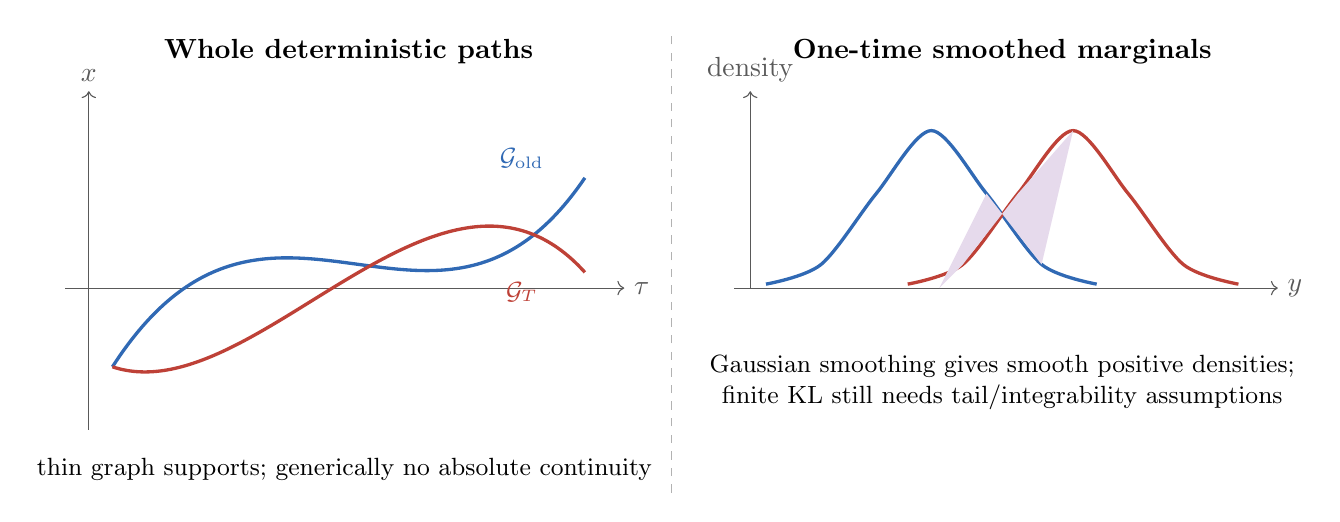
\begin{tikzpicture}[x=1cm,y=1cm]
  \node[font=\bfseries] at (0,3.0) {Whole deterministic paths};
  \draw[->,black!65] (-3.6,0) -- (3.5,0) node[right] {$\tau$};
  \draw[->,black!65] (-3.3,-1.8) -- (-3.3,2.5) node[above] {$x$};
  \draw[very thick,oldblue] (-3.0,-1.0) .. controls (-1.0,2.1) and (1.1,-1.4) .. (3.0,1.4);
  \draw[very thick,teacherred] (-3.0,-1.0) .. controls (-1.2,-1.6) and (1.2,2.2) .. (3.0,0.2);
  \node[text=oldblue,font=\small] at (2.2,1.65) {$\mathcal G_{\old}$};
  \node[text=teacherred,font=\small] at (2.2,-0.05) {$\mathcal G_T$};
  \node[align=center,font=\small] at (0,-2.3) {
    thin graph supports; generically no absolute continuity
  };

  \draw[dashed,black!30] (4.1,-2.6)--(4.1,3.3);

  \begin{scope}[xshift=8.3cm]
    \node[font=\bfseries] at (0,3.0) {One-time smoothed marginals};
    \draw[->,black!65] (-3.4,0)--(3.5,0) node[right] {$y$};
    \draw[->,black!65] (-3.2,0)--(-3.2,2.5) node[above] {density};
    \draw[very thick,oldblue,smooth] plot coordinates {
      (-3,0.05) (-2.3,0.3) (-1.6,1.2) (-0.9,2.0) (-0.2,1.2) (0.5,0.3) (1.2,0.05)
    };
    \draw[very thick,teacherred,smooth] plot coordinates {
      (-1.2,0.05) (-0.5,0.3) (0.2,1.2) (0.9,2.0) (1.6,1.2) (2.3,0.3) (3,0.05)
    };
    \fill[targetpurple!20] (-0.8,0)--(-0.5,0.3)--(0.2,1.2)--(0.9,2.0)
      --(0.5,0.3)--(-0.2,1.2)--cycle;
    \node[align=center,font=\small] at (0,-1.2) {
      Gaussian smoothing gives smooth positive densities;\\
      finite KL still needs tail/integrability assumptions
    };
  \end{scope}
\end{tikzpicture}
}
\caption{Distinct deterministic path graphs are generically singular, even when their one-time
marginals overlap.  MoD-TDM therefore matches Gaussian-smoothed marginals, not deterministic
path laws.}
\label{fig:path-singularity}
\end{figure}

Branch-fixed source trajectories remain the correct way to sample each $q_{k,\tau}$ jointly and
efficiently.  Matching all one-time marginals does not imply that the student's path law equals
the old/teacher path mixture: many processes share the same marginal family, and the learned
student is one deterministic flow.

\section{Proximal and contraction interpretation}
\label{sec:contraction}

\subsection{Ideal outer recursion}

Suppose each outer solve is exact at a fixed $\tau$:
\begin{equation}
\rho_{k+1,\tau}
=(1-\alpha_k)\rho_{k,\tau}+\alpha_k\rho_{T,\tau}.
\label{eq:outer-recursion}
\end{equation}
Assume $\alpha_k\in[0,1]$, the displayed KL terms are finite, and both laws have finite
$p$th moments for $p\ge1$.
Let $A_K=\prod_{j=0}^{K-1}(1-\alpha_j)$.  Induction gives
\begin{equation}
\rho_{K,\tau}=A_K\rho_{0,\tau}+(1-A_K)\rho_{T,\tau}.
\label{eq:outer-closed-form}
\end{equation}
For $\TV(\mu,\nu)=\frac12\norm{\mu-\nu}_1$,
\begin{align}
\TV(\rho_{k+1,\tau},\rho_{T,\tau})
&=(1-\alpha_k)\TV(\rho_{k,\tau},\rho_{T,\tau}),
\label{eq:tv-contraction}\\
\KL(\rho_{k+1,\tau}\Vert\rho_{T,\tau})
&\le(1-\alpha_k)\KL(\rho_{k,\tau}\Vert\rho_{T,\tau}),
\label{eq:kl-contraction}\\
\W_p^p(\rho_{k+1,\tau},\rho_{T,\tau})
&\le(1-\alpha_k)\W_p^p(\rho_{k,\tau},\rho_{T,\tau}).
\label{eq:wasserstein-contraction}
\end{align}
The KL inequality is convexity in the first argument.  The Wasserstein bound couples the
teacher component to itself and transports only old mass.

\subsection{Fitting-error bound and Pinsker}

Let the actual fitted law $\widehat\rho_{k+1,\tau}$ satisfy
\[
\varepsilon_{k,\tau}
:=\TV(\widehat\rho_{k+1,\tau},q_{k,\tau}).
\]
Then
\begin{equation}
\TV(\widehat\rho_{k+1,\tau},\rho_{T,\tau})
\le
\varepsilon_{k,\tau}
+(1-\alpha_k)\TV(\rho_{k,\tau},\rho_{T,\tau}).
\label{eq:fitting-tv}
\end{equation}
Iterating yields
\begin{equation}
D_K
\le A_KD_0+
\sum_{j=0}^{K-1}
\left[\prod_{\ell=j+1}^{K-1}(1-\alpha_\ell)\right]\varepsilon_j,
\label{eq:iterated-error}
\end{equation}
where $D_k=\TV(\rho_{k,\tau},\rho_{T,\tau})$.
If one separately certifies the \emph{unsmoothed} bound
$\KL(\widehat\rho_{k+1,\tau}\Vert q_{k,\tau})\le\delta_{k,\tau}$, Pinsker gives
\begin{equation}
\varepsilon_{k,\tau}\le\sqrt{\delta_{k,\tau}/2}.
\label{eq:pinsker}
\end{equation}
This unsmoothed certificate does not follow from a small value of the proposed Gaussian-smoothed
objective: data processing gives
\[
\KL((K_s)_\#p\Vert(K_s)_\#q)\le\KL(p\Vert q),
\]
which is the opposite direction.  At a fixed smoothing level one obtains only
\[
\TV(\widehat\rho_{k+1,\tau,s},q_{k,\tau,s})
\le
\sqrt{\KL(\widehat\rho_{k+1,\tau,s}\Vert q_{k,\tau,s})/2}.
\]
Exact equality after an informative Gaussian convolution with $a_s\ne0$ identifies the
unsmoothed law, but approximate deconvolution is unstable without additional regularity.

\begin{tcolorbox}[colback=red!4,colframe=red!45!black,title=What reverse KL does and does not inherit]
The ideal mixture recursion has exact TV contraction and the stated KL/Wasserstein upper bounds.
Smoothed reverse-KL training inherits unsmoothed outer contraction only with a separate
unsmoothed fitting guarantee or additional stability assumptions.  With finite capacity,
reverse KL may mode-select inside $q_k$; then fitting error can dominate the ideal contraction.
\end{tcolorbox}

\section{Score errors, lag, and source choices}
\label{sec:errors}

\subsection{Target lag versus fake lag}

The target-mixture score should be trained from the frozen old/teacher source and then held fixed
for one outer inner loop.  Its lag is an \emph{outer-target approximation} error.  The fake score
tracks the changing live student and therefore has \emph{online lag}.  Mixing these update
semantics destroys the frozen-target interpretation.

Let
\[
\widehat\score_q=\score_q+e_q,\qquad
\widehat\score_{\fake}=\score_{\fake}+e_{\fake}.
\]
The generator-gradient bias obeys
\begin{equation}
\norm{\operatorname{Bias}}
\le
\E\!\left[
\bar\lambda(s)|a_s|\norm{J_\theta}
\bigl(\norm{e_{\fake}}+\norm{e_q}\bigr)
\right].
\label{eq:score-bias-bound}
\end{equation}
This directly motivates target holdout DSM loss, fake freshness ratios, and score-difference
norm diagnostics.

\subsection{Classifier-error amplification}

For route B, let $\widehat\gamma=\gamma+\delta_\gamma$ and source score errors be
$e_{\old},e_T$.  Then
\begin{align}
\widehat\score_q-\score_q
&=\delta_\gamma(\score_T-\score_{\old})
 +(1-\widehat\gamma)e_{\old}+\widehat\gamma e_T.
\label{eq:classifier-error}
\end{align}
Even a small $\delta_\gamma$ is dangerous where the source scores are far apart.  Low-overlap
regions also produce extreme class probabilities and poor calibration.

\subsection{Rollout-old is not the fixed pretrained base}

The proximal source must be $\theta_k$, refreshed at the outer boundary.  Replacing it by a
fixed pretrained base $\rho_B$ changes the target to
$(1-\alpha)\rho_B+\alpha\rho_T$ every time and removes recursion
\eqref{eq:outer-recursion}.  A deliberate three-way target is possible:
\begin{equation}
q_{k,\tau}
=(1-\alpha-\beta)\rho_{\old,\tau}
+\alpha\rho_{T,\tau}
+\beta\rho_{B,\tau},
\qquad \alpha,\beta\ge0,\quad\alpha+\beta\le1.
\label{eq:three-way}
\end{equation}
It should be named and analyzed as a three-source anchor, not silently implemented by confusing
old with base.

\section{Implementation blueprint for Flow-Factory}
\label{sec:implementation}

\subsection{Five network/source roles}

\begin{figure}[htbp]
\centering
\resizebox{\textwidth}{!}{
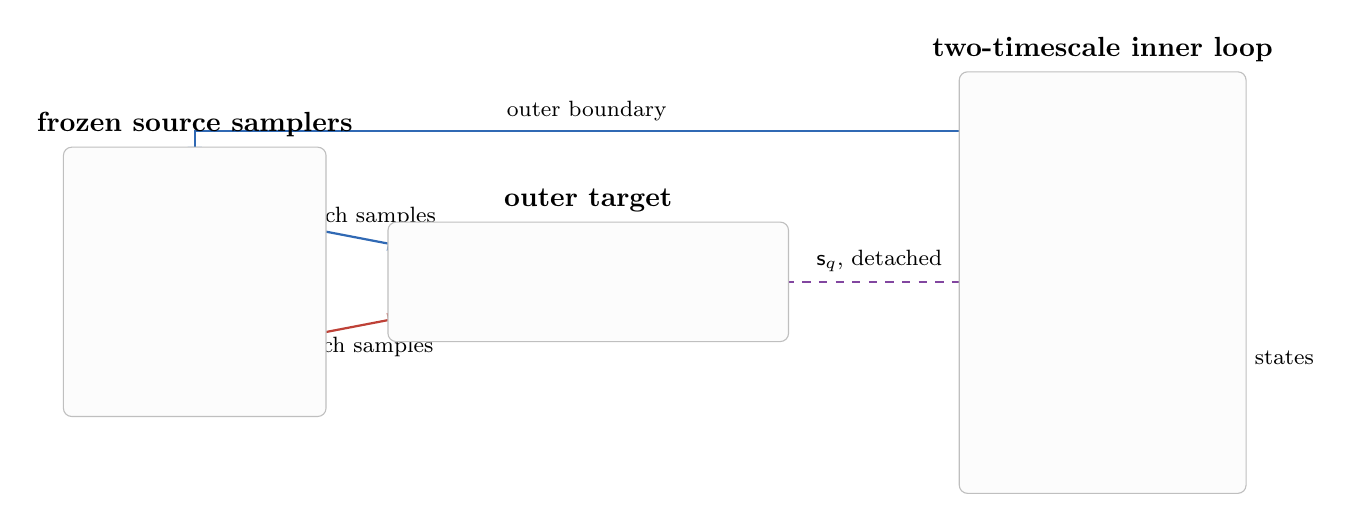
\begin{tikzpicture}[node distance=9mm and 14mm]
  \node[oldbox] (old) {rollout-old source\\frozen $\theta_k$};
  \node[teacherbox,below=of old] (teacher) {teacher source\\frozen};
  \node[targetbox,right=27mm of $(old)!0.5!(teacher)$] (target) {
    target-mixture score\\trained, then frozen per outer
  };
  \node[studentbox,right=28mm of target] (student) {
    student generator\\trainable $\theta$
  };
  \node[fakebox,below=of student] (fake) {
    online fake score\\trainable $\phi$
  };
  \node[neutralbox,above=of student] (eval) {evaluation / refresh\\old $\leftarrow$ student};

  \draw[flowarrow,draw=oldblue] (old) -- node[above,font=\footnotesize] {branch samples} (target);
  \draw[flowarrow,draw=teacherred] (teacher) -- node[below,font=\footnotesize] {branch samples} (target);
  \draw[detacharrow,draw=targetpurple] (target) -- node[above,font=\footnotesize] {$\score_q$, detached} (student);
  \draw[flowarrow,draw=fakeorange] (student) -- node[right,font=\footnotesize] {detached live states} (fake);
  \draw[detacharrow,draw=fakeorange] (fake) -- node[below,font=\footnotesize] {$\score_{\fake}$, detached} (student);
  \draw[flowarrow,draw=studentgreen] (student) -- (eval);
  \draw[flowarrow,draw=oldblue] (eval.west) -| node[pos=0.25,above,font=\footnotesize] {outer boundary} (old.north);

  \node[panel,fit=(old)(teacher),label={[font=\bfseries]above:frozen source samplers}] {};
  \node[panel,fit=(target),label={[font=\bfseries]above:outer target}] {};
  \node[panel,fit=(student)(fake)(eval),label={[font=\bfseries]above:two-timescale inner loop}] {};
\end{tikzpicture}
}
\caption{Proposed roles and update loops.  Old and fake are distinct: old defines the frozen
proximal target; fake estimates the moving current student's score.}
\label{fig:network-roles}
\end{figure}

\subsection{Conceptual pseudocode}

\begin{lstlisting}[style=goodpython,caption={Proposed outer/inner structure; names are conceptual, not accepted config/API fields.}]
old_source.load_snapshot(student.state_dict())  # conceptual API

# Phase A: fit q_k score from branch-fixed source trajectories.
for source_batch in target_score_batches:
    branch = collective_safe_bernoulli(alpha, shape=source_batch.shape)
    trajectory = rollout_selected_frozen_source_once(
        old_source=old_source,
        teacher_source=teacher_source,
        branch=branch,
    )
    tau_q = sample_target_trajectory_time()  # 1.0 for endpoint MoD-DMD
    X_q = trajectory.state_at(tau_q).detach()
    s_q, eps_q = sample_auxiliary_corruption(X_q)
    Y_q = a(s_q) * X_q + b(s_q) * eps_q
    loss_target = mse(target_score.aux_velocity(Y_q, tau_q, s_q),
                      eps_q - X_q)
    update_target_score_only(loss_target)
target_score.freeze()

# Phase B: two-timescale current-student updates.
for inner_step in inner_steps:
    X_live, tau_live = rollout_student_with_requested_jacobian()

    # Fake trains on detached live states.
    s_f, eps_f = sample_auxiliary_corruption(X_live.detach())
    Y_f = a(s_f) * X_live.detach() + b(s_f) * eps_f
    loss_fake = mse(fake_score.aux_velocity(Y_f, tau_live, s_f),
                    eps_f - X_live.detach())
    update_fake_only(loss_fake)

    # Generator sees detached scores, but X_live keeps its sampler graph.
    s_g, eps_g = sample_auxiliary_corruption(X_live.detach())
    with torch.no_grad():
        Y_value = a(s_g) * X_live.detach() + b(s_g) * eps_g
        score_q = target_score.score(Y_value, tau_live, s_g)
        score_fake = fake_score.score(Y_value, tau_live, s_g)
        force = importance_weight(tau_live, s_g) * a(s_g) \
              * (score_fake - score_q)
    loss_gen = stop_gradient_force_loss(X_live, force)
    update_student_only(loss_gen)
\end{lstlisting}

\begin{lstlisting}[style=badpython,caption={Wrong detach and role combinations.}]
# WRONG 1: moving target; q_k is no longer frozen.
update_target_score_on_live_student_states()

# WRONG 2: old and fake are not interchangeable.
score_fake = old_source.predict_velocity(tau, X_live)

# WRONG 3: score networks enter generator backward.
loss = ((fake_score(Y) - target_score(Y)) * X_live).sum()

# WRONG 4: branch redraw inside the source ODE loop.
for step in source_trajectory_steps:
    branch = torch.rand(batch_size) < alpha
\end{lstlisting}

\subsection{Endpoint and TDM data flow}

Endpoint MoD-DMD needs target source states only at $\tau=1$, plus live student endpoints.
MoD-TDM needs source and live-student states at sampled $\tau_i$.  A practical first version can
store selected source states/callbacks and train the target score offline within each outer
iteration.  The generator may begin with one randomly selected, rank-broadcast segment and a
one-step truncated Jacobian, clearly labeled as an approximation to
\eqref{eq:mod-tdm-objective}.

Current \texttt{XTrajectoryDMTrainer} subclasses---\texttt{XTDMTrainer} and
\texttt{XOPDDMTrainer}---have an additional v1 mismatch worth logging explicitly.  Their
generator query uses the selected segment band, but the shared fake update trains on a
full-rollout endpoint with auxiliary noise sampled globally over $[0,1]$.  A strict
segment-conditioned implementation should verify that fake training estimates the same
$p_{\theta,u}^{(i)}$ queried by the generator, or document the endpoint-trained fake as a
surrogate.

\subsection{Configuration concepts, not invented accepted fields}

A future configuration design needs concepts for:
\begin{itemize}[leftmargin=1.5em]
\item algorithm mode (endpoint MoD-DMD versus multi-time MoD-TDM);
\item outer mixture weight or schedule, and old-refresh cadence;
\item target-score architecture, optimizer, training steps, and freeze boundary;
\item fake-score optimizer and fake-to-generator update ratio;
\item $\tau$ grid or sampling law, auxiliary $s$ law, and exact importance weights;
\item sampler-gradient mode (full BPTT, checkpointed BPTT, or one-step truncation);
\item event reduction, optional self-normalization, and optional Pseudo-Huber metric.
\end{itemize}
These are design requirements, not claims about existing Pydantic field names.  Exact fields
must be introduced through the normal training-argument synchronization and config-validation
process.

Existing fields that provide nearby, but not sufficient, mechanics include:
\begin{itemize}[leftmargin=1.5em,nosep]
\item \texttt{xopd\_target\_mode: marginal\_cfm} and
      \texttt{marginal\_cfm\_alpha};
\item \texttt{dmd\_fake\_ratio} and \texttt{tdm\_fake\_ratio};
\item \texttt{tdm\_match\_policy: random\_segment};
\item \texttt{tdm\_loss\_metric: pseudo\_huber}.
\end{itemize}
None currently activates a mixture-target score.

\subsection{Diagnostics}

At minimum, log:
\begin{itemize}[leftmargin=1.5em]
\item realized old/teacher branch fractions by rank and globally;
\item target DSM train/holdout losses by $(\tau,s)$ and source branch;
\item fake DSM loss, fake age, and fake-to-generator update ratio;
\item $\norm{\score_{\fake}-\score_q}$ and denoiser residual quantiles by $(\tau,s)$;
\item generator force norm before/after normalization, gradient norm, and clipping rate;
\item selected segment histogram and exact $w_i/\pi_i$ weights;
\item old--teacher, current--target, and current--teacher sample metrics;
\item target refresh number, inner step, and whether the Jacobian was full or truncated.
\end{itemize}

\subsection{Distributed and mixed-precision invariants}

\begin{enumerate}[leftmargin=1.6em]
\item \textbf{Rank-synchronous source call order.}  Branch routing must make every rank enter old
      and teacher collectives in the same order.  Synchronize branch geometry or execute both
      branch calls with collective-safe padding.
\item \textbf{Identical branch labels across ranks.}  The Bernoulli RNG key must exclude rank
      and use shared values such as seed, epoch, and batch index, as in
      \texttt{draw\_marginal\_cfm\_branches}.  Otherwise subset shapes and teacher collectives can
      diverge across ranks.
\item \textbf{Broadcast the segment index.}  A random TDM segment changes the number of prefix
      transformer calls; draw on one rank and broadcast before rollout.
\item \textbf{Current teacher-real swap.}  The shipped FLUX.2-Klein
      \texttt{use\_teacher\_transformer} context swaps the whole module, bypasses the wrapped
      student for the no-grad teacher forward, and already disables/restores the autocast cache.
\item \textbf{Future copied-weight old snapshots.}  Any no-grad loop using either of these
      copied-weight swap contexts,
      \par\smallskip
      \path{adapter.use_named_parameters(name)}
      \par
      \path{EMAModuleWrapper.use_ema_parameters(),}
      \par\smallskip
      must disable the autocast weight cache for the full swap loop and restore its prior value
      afterward.
\item \textbf{DDP bypass for copied weights.}  A no-grad named-parameter weight swap must
      temporarily route the transformer component through its unwrapped module.  DDP parameter
      buckets can otherwise expose stale weights after \texttt{.data.copy\_()} swaps.
\item \textbf{Training exception.}  The gradient-enabled student pass remains through the prepared
      DDP/DeepSpeed wrapper so gradients synchronize correctly.
\item \textbf{Manual fake optimizer.}  If fake parameters are added after
      \path{accelerator.prepare}, gradients must be explicitly all-reduced and replicas
      initialized identically, as in the current implementations.
\end{enumerate}

\subsection{Exact mapping to current files and the gap}

\begin{center}
\small
\begin{tabular}{@{}
  >{\raggedright\arraybackslash}p{0.30\textwidth}
  >{\raggedright\arraybackslash}p{0.29\textwidth}
  >{\raggedright\arraybackslash}p{0.32\textwidth}
@{}}
\toprule
current file / symbol & what it does now & required MoD change\\
\midrule
\path{trainers/xopd/trainer.py}: \texttt{XOPDTrainer} \texttt{marginal\_cfm}
& A4 branch-fixed old/teacher source rollout and source-velocity MSE
& reuse branch routing/call order for target-score data; add the target-score phase and an
  explicit freeze boundary; current $B=0$ is the rollout-time student, not a separately
  materialized snapshot\\
\addlinespace
\path{trainers/xopd/dmd_trainer.py}: \texttt{XDMDTrainer}
& endpoint DMD; \texttt{real}=teacher, online \texttt{fake}=student score; consistency-style
  no-grad prefix plus one differentiable prediction
& replace teacher-only real score by a learned frozen-per-outer
  $q_{k,1,s}$ score and add rollout-old snapshot/refresh\\
\addlinespace
\path{trainers/xopd/traj_dm_trainer.py}: \texttt{XTDMTrainer}
& random rank-broadcast segment; no-grad prefix plus one differentiable Euler step; teacher real
  score; detached live state re-noised as a clean target
& learn $q_{k,\tau_i,s}$, preserve two clocks, use exact random-time weights, and label
  one-step Jacobian as truncated\\
\addlinespace
\path{trainers/xopd/traj_dm_trainer.py}: \texttt{XOPDDMTrainer}
& same random-segment score-difference recipe on the OPD
  \texttt{num\_inference\_steps} grid
& the same mixture-target changes as XTDM; keep its grid distinction explicit\\
\addlinespace
\path{trainers/xopd/traj_dm.py}
& RF corruption, clean-estimate conversion, self-normalized force, stop-grad/Pseudo-Huber helpers,
  signed Euler update
& retain useful mechanics but add mathematically explicit $a_s,b_s,\lambda(s)$ weighting and
  target-mixture interfaces\\
\bottomrule
\end{tabular}
\end{center}

Current \texttt{XDMDTrainer} computes teacher and fake predictions at an auxiliary-noised live
endpoint, then uses a self-normalized clean-estimate residual.  Current
\texttt{XTDMTrainer} samples one segment, executes a no-grad prefix, differentiates one Euler
step, and uses the teacher as real.  Neither constructs
\[
(1-\alpha)\rho_{\theta_k,\tau,s}+\alpha\rho_{T,\tau,s}.
\]
Current TDM v1 does not compute the exact gradient of
\eqref{eq:mod-tdm-objective}.  Uniform random-segment sampling is unbiased up to an overall
constant for equal segment weights, but the one-step truncated Jacobian, self-normalization, and
optional Pseudo-Huber metric produce a semi-gradient rather than exact full BPTT.

\section{Compact comparison}
\label{sec:comparison}

\begin{center}
\scriptsize
\setlength{\tabcolsep}{3.2pt}
\begin{tabular}{@{}
  >{\raggedright\arraybackslash}p{0.13\textwidth}
  >{\raggedright\arraybackslash}p{0.17\textwidth}
  >{\raggedright\arraybackslash}p{0.18\textwidth}
  >{\raggedright\arraybackslash}p{0.17\textwidth}
  >{\raggedright\arraybackslash}p{0.24\textwidth}
@{}}
\toprule
method & probability target & target signal & generator Jacobian & status / defining distinction\\
\midrule
A4 CFM
& $q_{k,\tau}$ marginal path
& sampled source ODE velocity
& $\partial_\theta v_\theta$ at sampled state
& implemented as XOPD \texttt{marginal\_cfm}; density mixture without DMD fake score\\
\addlinespace
ordinary XDMD
& teacher endpoint density
& teacher score minus online fake score
& one differentiable consistency prediction
& implemented; teacher is real, no old/teacher mixture\\
\addlinespace
\textbf{proposed MoD-DMD}
& $q_{k,1}$ endpoint mixture
& frozen mixture score minus online fake score
& endpoint sampler $J_\theta$
& new outer-target algorithm; not implemented\\
\addlinespace
ordinary XTDM
& teacher-real score surrogate on selected student states
& teacher score minus online fake score
& v1 no-grad prefix + one Euler step
& implemented random-segment truncated semi-gradient, not full sum\\
\addlinespace
\textbf{proposed MoD-TDM}
& $q_{k,\tau_i}$ multi-marginals, native $q_{k,u}$, or symmetric
  $\widetilde q_{k,u}^{(i)}$ segments
& frozen mixture score minus online fake score
& exact BPTT or declared truncation
& new multi-time/segment smoothed reverse KL; not implemented\\
\bottomrule
\end{tabular}
\end{center}

\section{Limitations and recommended implementation order}
\label{sec:limitations}

\subsection{Limitations}

\begin{itemize}[leftmargin=1.5em]
\item A learned target-mixture score adds memory, compute, and an outer fitting phase.
\item Teacher source trajectories remain expensive; branch sampling reduces expected cost but
      does not eliminate teacher rollout.
\item Low old/teacher overlap weakens the first-step teacher force under reverse KL.
\item Auxiliary smoothing trades overlap and score learnability against fine-detail fidelity.
\item Fake-score lag can destabilize the generator; target and fake errors enter the same force.
\item Finite-capacity reverse KL may mode-select instead of representing the convex mixture.
\item Full multi-time BPTT can be prohibitively expensive; truncation introduces bias.
\item Cross-VAE settings need an explicit common state/noise space before any mixture density is
      meaningful.
\item Matching marginal families does not identify or match a deterministic path law.
\end{itemize}

\subsection{Recommended implementation order}

\begin{enumerate}[leftmargin=1.6em]
\item Build a CPU/test-only mathematical harness for Gaussian mixtures that verifies
      \eqref{eq:mixture-score}, \eqref{eq:rf-score}, \eqref{eq:pathwise-gradient}, and
      \eqref{eq:first-force} by finite differences.
\item Implement endpoint target-mixture DSM data using the existing A4 branch-fixed source
      routing; keep the target network separate and frozen per outer loop.
\item Replace XDMD's teacher-only real score behind a new explicitly named experimental mode;
      preserve ordinary XDMD unchanged.
\item Add detach, update-ratio, distributed call-order, autocast-cache, and DDP-bypass tests.
\item Validate endpoint MoD-DMD on a same-VAE, small-resolution setup with exact unnormalized
      weighting before introducing self-normalization or Pseudo-Huber.
\item Extend target-score conditioning to trajectory time $\tau$ and verify random-time importance
      weights.
\item Add MoD-TDM first with current one-step truncation, naming and logging it as such; compare
      against short-horizon full BPTT on tiny models.
\item Only then study dynamic $\alpha_k$, three-way anchors, cross-VAE transport, or classifier
      routing.
\end{enumerate}

\section{Internal documents and final checklist}
\label{sec:references}

The closest internal references are:
\begin{itemize}[leftmargin=1.5em]
\item \href{run:../core/marginal_cfm/arm_a4_marginal_mixture_cfm_tutorial.pdf}
      {\path{docs/xopd/core/marginal_cfm/arm_a4_marginal_mixture_cfm_tutorial.pdf}} for A4;
\item \href{run:../xdmd/dmd_opd_gradient_relation.pdf}
      {\path{docs/xopd/xdmd/dmd_opd_gradient_relation.pdf}} for OPD versus endpoint DMD;
\item \href{run:../trajectory_dm/tdm_opd_dm_gradient_relation.tex}
      {\path{docs/xopd/trajectory_dm/tdm_opd_dm_gradient_relation.tex}} for current TDM Jacobians;
\item \href{run:../core/p_opd/popd_exact_sum_gate_saturation.pdf}
      {\path{docs/xopd/core/p_opd/popd_exact_sum_gate_saturation.pdf}} for transition-gate behavior;
\item \href{run:../flow_direct_opd/flow_direct_opd_small_rl_delta_transfer.pdf}
      {\path{docs/xopd/flow_direct_opd/flow_direct_opd_small_rl_delta_transfer.pdf}} for direct OPD context.
\end{itemize}

\begin{tcolorbox}[colback=green!5,colframe=green!50!black,title=Minimum mathematically faithful MoD implementation]
\begin{enumerate}[leftmargin=1.5em]
\item[$\checkmark$] Old means frozen $\theta_k$, not current and not fixed pretrained base.
\item[$\checkmark$] Source branch is sampled once per complete trajectory.
\item[$\checkmark$] $\tau$ and $s$ are stored and conditioned separately.
\item[$\checkmark$] Target score represents $q_{k,\tau,s}$, not teacher alone.
\item[$\checkmark$] Fake score trains on detached live-student states.
\item[$\checkmark$] Generator sign is $\score_{\fake}-\score_q$; descent moves toward
      $\score_q-\score_{\fake}$.
\item[$\checkmark$] Denoiser form includes $a_s^2/b_s^2$, or changed weighting is disclosed.
\item[$\checkmark$] Target and fake scores are detached in generator backward.
\item[$\checkmark$] Random-time weights and scheduler orientation are explicit.
\item[$\checkmark$] Truncated Jacobians are not described as exact BPTT.
\item[$\checkmark$] Claims concern smoothed marginals, not deterministic path-space KL.
\item[$\checkmark$] Distributed named-parameter swaps obey call-order, autocast-cache, and DDP
      invariants.
\end{enumerate}
\end{tcolorbox}

\section{Conclusion}

MoD-DMD and MoD-TDM combine two ideas without conflating their mathematical objects.  A4 supplies
a frozen old/teacher \emph{density target} in the outer-loop mathematical sense; shipped
\texttt{marginal\_cfm} instead uses the rollout-time student on the $B=0$ branch and caches its
velocity target.  DMD/TDM supply a score-difference
\emph{distribution-matching update}.  Gaussian smoothing makes the target score learnable,
branch-fixed source sampling avoids explicit density estimation, and the online fake score
provides the entropy side of reverse KL.  The exact endpoint force is
\[
a_sJ_\theta^\top(\score_{\fake}-\score_q),
\]
and the first inner step is gated by the smoothed posterior responsibility.  Multi-time matching
may use independently smoothed ODE marginals or the paper-style segment-conditioned laws in
\eqref{eq:segment-mod-tdm}; these are distinct unless their kernels and marginal-consistency
identities agree.  In either case, sampler sensitivity---exact or explicitly truncated---carries
the score force to parameters.

The practical boundary is equally important: current XDMD and XTDM are teacher-real methods.
Turning them into MoD methods requires a frozen rollout-old source, a separately trained
old/teacher target-mixture score, an outer refresh protocol, and new diagnostics and invariants.
Changing a label from ``teacher'' to ``mixture'' or averaging source velocities would not
implement the proposal.

\begin{thebibliography}{9}

\bibitem{flowmatching}
Yaron Lipman, Ricky T. Q. Chen, Heli Ben-Hamu, Maximilian Nickel, and Matt Le.
\newblock Flow Matching for Generative Modeling.
\newblock \emph{International Conference on Learning Representations}, 2023.
\newblock \url{https://arxiv.org/abs/2210.02747}.

\bibitem{diffinstruct}
Weijia Luo, Zhiwei Hu, Yijun Zhang, et al.
\newblock Diff-Instruct: A Universal Approach for Transferring Knowledge From Pre-trained
Diffusion Models.
\newblock \emph{Advances in Neural Information Processing Systems}, 2023.
\newblock \url{https://arxiv.org/abs/2305.18455}.

\bibitem{dmd}
Tianwei Yin, Micha\"el Gharbi, Richard Zhang, Eli Shechtman, Fr\'edo Durand,
William T. Freeman, and Taesung Park.
\newblock One-step Diffusion with Distribution Matching Distillation.
\newblock \emph{CVPR}, 2024.
\newblock \url{https://arxiv.org/abs/2311.18828}.

\bibitem{dmd2}
Tianwei Yin, Micha\"el Gharbi, Taesung Park, Richard Zhang, Eli Shechtman,
Fr\'edo Durand, and William T. Freeman.
\newblock Improved Distribution Matching Distillation for Fast Image Synthesis.
\newblock \emph{NeurIPS}, 2024.
\newblock \url{https://arxiv.org/abs/2405.14867}.

\bibitem{tdm}
Weijian Luo et al.
\newblock Learning Few-Step Diffusion Models by Trajectory Distribution Matching.
\newblock \emph{ICCV}, 2025.
\newblock \url{https://arxiv.org/abs/2503.06674}.

\bibitem{tweedie}
Bradley Efron.
\newblock Tweedie's Formula and Selection Bias.
\newblock \emph{Journal of the American Statistical Association}, 2011.
\newblock \url{https://doi.org/10.1198/jasa.2011.tm11181}.

\end{thebibliography}

\end{document}
